% Chapter 4

\chapter{Project Simulation} % Write in your own chapter title
\label{Chapter4}
\lhead{} % Write in your own chapter title to set the page header

\section{Simulation Setup}
% Simply detail the hyperparameters/learnables parameters in both convmc, original hubermc and later hubermc. also mention the loss (MSE vs specific L0-BCD val loss). Take some of intepretation of the compilation
We implemented both of our models using PyTorch and conducted numerous experiments in search of an optimal combination of parameters to meet our objectives. The following hyperparameters were chosen for training the ConvMC-Net model:
\begin{verbatim}
    layers = 5
    kernel = [[(3, 1)] * 3 + [(3, 1)] * 7][0:layers]
    stride = (1, 1)
    padding = (1, 1)
    initial_mu_inverse = 0.0
    initial_y1 = 0.8
    coef_mu_inverse = 0.36
    rank = 10
\end{verbatim}

For ConvHuberMC-Net, it was the following combination:
\begin{verbatim}
    layers = 3
    kernel = (3, 3)
    stride = (1, 1)
    padding = int((kernel - 1) / 2)
    hubreg_iters = 2
    rank = 10
\end{verbatim}

% Additional Points: Add padding and stride where conv operations are being used. obv include rank below as well 
% L0-BCD: mu/epsilon
% M-est: alpha and c
% ORMC: 500 maxiter, num_trials 1
% lp-admm(p = 1): 500 maxiter, num_trials 1
% lp-reg(p = 1): 1000 maxiter, num_trials 1
Here, \verb|layers| are the number of layers in the neural network, \verb|kernel| is the shape of the convolution kernel, \verb|initial_mu_inverse| is the regularization parameter, \verb|initial_y1| is the Lagrange multiplier, \verb|coef_mu_inverse| is the coefficient that scales the regularization parameter iteratively, \verb|rank| is the rank of the recovered matrix, and \verb|hubreg_iters| is the number of times Huber regression is performed in one layer.

Both of these models also had a shape parameter that was used to test our model on two shapes: (150 \(\times\) 300) and (400 \(\times\) 500). We used normalized mean squared error (NMSE) as our training loss because we found that to be more conducive to learning: \[\mathcal{L} = \frac{1}{N}\sum_{i = 1}^N\frac{\|L_i - \bar L_i\|}{\|L_i\|_F^2}\] where N is the total number of training sequences in the data set, L is output predicted by the network, and L is the ground-truth. For validation, however, we used the loss function used by \(\ell_0\)-BCD, simple mean squared error, to allow for a fair comparison: \[\text{MSE} = \frac{\|M - X\|_F^2}{mn}\] where M is the recovered matrix, X is the original matrix, and \((m \times n)\) is the shape of these two matrices.

As we compare our models with a number of different algorithms, it is apt to briefly mention the parameters we used for them too. They are listed in Table \ref{tab:params_net}.

\begin{table}[htbp]
    \centering
    \begin{tabular}{cc}
        \toprule
        \textbf{Algorithm} & \textbf{(Hyper)Parameters} \\
        \midrule
        \(\ell_0\)-BCD & \(\epsilon = 1e-20\) \\
        M-estimation & \(c = 1.345\) \\
        \(\ell_p\)-reg (p = 1) & maxiter = 1000, num\_trials = 1 \\
        \(\ell_p\)-ADMM (p = 1) & maxiter = 500, num\_trials = 1 \\
        ORMC & maxiter = 500, num\_trials = 1 \\
        ADMM-Net & \(\eta_0 = 1.81, \ \rho_0 = 0.1001, v_0 = 0\) \\
        \bottomrule
    \end{tabular}
    \caption{(Hyper)Parameters for other algorithms and models}
    \label{tab:params_net}
\end{table}

Specifically for ADMM-Net, we tested values for \(eta_0 \in [1, 2]\), \(\rho_0 \in [0.00099, 0.1001]\), and \(v_0 \in [0, 0.2]\) to finally settle on the values shown in the table.

\section{Simulation Results, Analyses, and Outlook}
% Put every data comparison with all other algorithms including convmc, later hubermc (synthetic + image inpainting). Maybe even add the 8 images image inpainting result table in terms of PNSR, SSIM and show their reconstructed images.
\begin{figure}[htbp]
    \centering
    \includesvg{mse_snr_150_300}
    \caption{MSE vs SNR: sampling rate = 0.4, shape = (150 \(\times\) 300)}
    \label{fig:mse_snr_150_300}
\end{figure}

\begin{figure}[htbp]
    \centering
    \includesvg{mse_snr_400_500}
    \caption{MSE vs SNR: sampling rate = 0.4, shape = (400 \(\times\) 500)}
    \label{fig:mse_snr_400_500}
\end{figure}

\begin{table}[htbp]
    \centering
    \rotatebox{90}{
    \begin{tabular}{|ccccccccc|}
        \hline
        \textbf{Image} & \textbf{Mask} & \textbf{Metric} & \textbf{\(\ell_0)\)-BCD} & \textbf{\(\ell_p)\)-reg} & \textbf{\(\ell_p)\)-ADMM} & \textbf{ORMC} & \textbf{M-Estimation} & \textbf{ConvMC-Net} \\
        \hline
        \multirow{2}{*}{Image-1} & \multirow{2}{*}{random} & PSNR & 18.0168 & \textbf{21.2846} & 17.5846 & 14.2193 & 20.1214 & 14.6764 \\
         &  & SSIM & 0.3152 & \textbf{0.3511} & 0.1869 & 0.1498 & 0.2828 & 0.0197 \\
        \hline
        \multirow{2}{*}{Image-2} & \multirow{2}{*}{random} & PSNR & 16.9121 & \textbf{18.7851} & 16.2755 & 14.3490 & 17.9068 & 28.4482 \\
         &  & SSIM & 0.2681 & \textbf{0.2986} & 0.2004 & 0.2139 & 0.2401 & 0.4547 \\
        \hline
        \multirow{2}{*}{Image-3} & \multirow{2}{*}{random} & PSNR & 15.6531 & \textbf{19.7035} & 15.3484 & 11.3027 & 18.7403 & 13.8781 \\
         &  & SSIM & 0.2300 & \textbf{0.2769} & 0.1741 & 0.0977 & 0.2213 & 0.0524 \\
        \hline
        \multirow{2}{*}{Image-4} & \multirow{2}{*}{random} & PSNR & 16.5880 & \textbf{18.2356} & 14.4972 & 11.8165 & 17.2024 & 12.2581 \\
         &  & SSIM & 0.2358 & \textbf{0.2778} & 0.1973 & 0.1385 & 0.2355 & 0.0258 \\
        \hline
        \multirow{2}{*}{Image-5} & \multirow{2}{*}{random} & PSNR & 20.0771 & \textbf{20.9231} & 17.4914 & 14.7859 & 20.8793 & 13.4158 \\
         &  & SSIM & 0.3506 & \textbf{0.3734} & 0.2045 & 0.1584 & 0.3045 & 0.0587 \\
        \hline
        \multirow{2}{*}{Image-6} & \multirow{2}{*}{random} & PSNR & 17.8750 & 21.0284 & 15.3678 & 13.9751 & \textbf{21.0675} & 12.8591 \\
         &  & SSIM & 0.2762 & \textbf{0.3100} & 0.1493 & 0.1243 & 0.2923 & 0.0549 \\
        \hline
        \multirow{2}{*}{Image-7} & \multirow{2}{*}{random} & PSNR & 18.5359 & \textbf{21.4101} & 16.8222 & 13.4270 & 20.9942 & 14.4267 \\
         &  & SSIM & 0.2887 & \textbf{0.3233} & 0.1772 & 0.1098 & 0.2893 & 0.0453 \\
        \hline
        \multirow{2}{*}{Image-8} & \multirow{2}{*}{random} & PSNR & 7.6655 & 16.5794 & 10.8466 & 9.3512 & 16.0630 & \textbf{37.3651} \\
         &  & SSIM & 0.1510 & 0.2106 & 0.1441 & 0.1110 & 0.1816 & \textbf{0.8352} \\
        \hline
    \end{tabular}}
    \caption{PSNR and SSIM of different algorithms on eight 150 x 300 images with 5dB salt-and-pepper noise}
    \label{tab:psnr_ssim_150_300}
\end{table}

\begin{table}[htbp]
    \centering
    \rotatebox{90}{
    \begin{tabular}{|ccccccccc|}
        \hline
        \textbf{Image} & \textbf{Mask} & \textbf{Metric} & \textbf{\(\ell_0\)-BCD} & \textbf{\(\ell_p\)-reg} & \textbf{\(\ell_p\)-ADMM} & \textbf{ORMC} & \textbf{M-Estimation} & \textbf{ConvMC-Net} \\
        \hline
        \multirow{2}{*}{Image-1} & \multirow{2}{*}{random} & PSNR & \textbf{23.3228} & 22.9612 & 20.9205 & 15.3217 & 21.1176 & 12.7777 \\
         &  & SSIM & \textbf{0.4845} & 0.4427 & 0.2764 & 0.1409 & 0.3402 & 0.0438 \\
        \hline
        \multirow{2}{*}{Image-2} & \multirow{2}{*}{random} & PSNR & \textbf{19.2602} & 19.1894 & 18.2118 & 15.7579 & 18.1707 & 12.1982 \\
         &  & SSIM & \textbf{0.3309} & 0.3240 & 0.2423 & 0.2547 & 0.2724 & 0.0412 \\
        \hline
        \multirow{2}{*}{Image-3} & \multirow{2}{*}{random} & PSNR & \textbf{22.5507} & 22.0577 & 20.0277 & 12.9958 & 20.3123 & 13.4528 \\
         &  & SSIM & \textbf{0.4012} & 0.3602 & 0.2311 & 0.1054 & 0.2799 & 0.0446 \\
        \hline
        \multirow{2}{*}{Image-4} & \multirow{2}{*}{random} & PSNR & \textbf{19.4893} & 19.3902 & 18.5176 & 12.8923 & 18.8606 & 10.9455 \\
         &  & SSIM & \textbf{0.3372} & 0.3226 & 0.2353 & 0.1379 & 0.2794 & 0.0355 \\
        \hline
        \multirow{2}{*}{Image-5} & \multirow{2}{*}{random} & PSNR & \textbf{23.4655} & 23.3291 & 20.9843 & 15.9237 & 21.7869 & 12.5822 \\
         &  & SSIM & \textbf{0.5054} & 0.4825 & 0.2757 & 0.1643 & 0.3756 & 0.0407 \\
        \hline
        \multirow{2}{*}{Image-6} & \multirow{2}{*}{random} & PSNR & \textbf{23.1620} & 22.8400 & 20.4106 & 15.5223 & 21.5492 & 13.4670 \\
         &  & SSIM & \textbf{0.4573} & 0.4256 & 0.2241 & 0.1565 & 0.3604 & 0.0535 \\
        \hline
        \multirow{2}{*}{Image-7} & \multirow{2}{*}{random} & PSNR & \textbf{24.5711} & 23.9382 & 21.4715 & 14.7422 & 23.3300 & 14.2580 \\
         &  & SSIM & \textbf{0.4820} & 0.4298 & 0.2465 & 0.1195 & 0.3975 & 0.0614 \\
        \hline
        \multirow{2}{*}{Image-8} & \multirow{2}{*}{random} & PSNR & \textbf{18.3704} & 18.0212 & 17.1763 & 10.8709 & 16.9391 & 12.7077 \\
         &  & SSIM & \textbf{0.2809} & 0.2534 & 0.1930 & 0.1342 & 0.1941 & 0.0730 \\
        \hline
    \end{tabular}}
    \caption{PSNR and SSIM of different algorithms on eight 400 x 500 images with 5dB salt-and-pepper noise}
    \label{tab:psnr_ssim_400_500}
\end{table}

% Intepret each graph/table above in detail - address on unfolded huber in the context of synthetic only. 
% To start of with the results we compare ConvMC and ADMM-Net 

\begin{figure}[htbp]
    \centering
    \includesvg[width=\textwidth]{sampling rate}
    \caption{NMSE against sampling rate}
    \label{fig:samplingrate}
\end{figure}

\begin{figure}[htbp]
    \centering
    \includesvg[width=\textwidth]{background_mag}
    \caption{NMSE agiainst noise}
    \label{fig:background_mag}
\end{figure}

\begin{table}[htbp]
    \centering
    \begin{tabular}{ccc}
        \toprule
        \textbf{Model} & \textbf{Training time} & \textbf{Testing time} \\
        \midrule
        ConvMC-Net & \textbf{0.02283} & \textbf{0.01425} \\
        ADMM-Net & 0.4245 & 0.2629 \\
        \bottomrule
    \end{tabular}
    \caption{Training and testing time per sample for ADMM-Net and ConvMC-Net}
    \label{tab:time}
\end{table}

\textbf{Experiment settings:} We compare the performance of ConvMC-Net with ADMM-Net, both composed of five layers, on a real-world sensing data set that consists of temperature data collected every 30 seconds by 54 sensors distributed in Intel Berkeley Research Lab during February 28, 2004 and April 5, 2004. 468 such ground truth low-rank matrices L, each of shape (49 \(\times\) 60) and corrupted by zero-mean Gaussian noise, are created from this time series data set. Each row in L represents the successive readings of a sensor. Using a uniform probability density function, we randomly take out Q \(\cdot\) M \(\cdot\) N entries from L to create the incomplete matrix \(D_\Omega\). Q is the sampling rate defined as Q = card(\(\Omega\))/(M \(\cdot\) N), where card(\(\cdot\)) denotes the cardinality of a set. The first 400 matrices, consisting of the first (400 \(\times\) 49 \(\times\) 60) temperature recordings, are used for training both ConvMC-Net and ADMM-Net and the remaining 68 matrices are used for testing. Furthermore, both networks are trained for 40 epochs using ADAM optimizer with a learning rate of 0.01.

{Results:} Figure \ref{fig:samplingrate} shows the average NMSE loss \(\mathcal{L}\) obtained by both ConvMC-Net and ADMM-Net as Q increases from 0.2 to 0.6. As expected, \(\mathcal{L}\) decreases for both ConvMC-Net and ADMM-Net as Q increases. However, for lower values of Q, which makes matrix completion much more challenging, ConvMC-Net gives a lower loss than ADMM-Net. Figure \ref{fig:background_mag} shows the loss obtained by the two networks plotted against the noise power of the zero-mean Gaussian noise added to the data set. We observe that, as the noise power increases, the loss given by ADMM-Net also increases, whereas the loss given by ConvMC-Net increases only marginally. This improved robustness can be attributed to the learnable kernels introduced in the unfolding process of ConvMC-Net, unlike ADMM-Net, which only learns its tunable parameters from data.

Perhaps the biggest advantage of ConvMC-Net is that it takes significantly less time both in training and at inference than that taken by ADMM-Net as shown in Table \ref{tab:time}. This is because ADMM-Net in involves computing the inverse of (MN \(\times\) MN)-shaped matrix at every layer, resulting in much greater computation time. This also limits ADMM-Net's applicability on high-dimensional matrices, as large amount of RAM would be needed to calculate and store these inverses. The aforementioned advantages of ConvMC-Net, particularly that of less training and inference time, together with less computational burden, makes it an attractive candidate for real-time online applications on hardware constrained resources.

We conclude that when ADMM-Net is pitted against ConvMC-Net, particularly when it comes to dealing with white noise, ConvMC-Net wins because of its amazing inference time and accuracy. For this reason we exclude ADMM-Net in our future experiments and consider state-of-the-art algorithms that deal with impulsive GMM noise, which, according to the ADMM-Net formulation, cannot be handled by it because of the objective function being simply X = D + N, where N is the noise and we can clearly see that N is not explicitly broken down into sparse and dense noise components. This is not the case for other algorithms included in this paper.

% 4 Plots in total, i) HuberMC + ConvMC with all other algorithms synthetic plot for 150 x 300 ii) HuberMC + ConvMC with all other algorithms synthetic plot for 400 x 500 iii) ConvMC with all other algorithms Image inpainting perfromance on 150 x 300, and iv) for 400 x 500 same as iii)

% For e.g take the first graph. Choose a combination fixing sampling rate and varying DB on the basis of certain factors which you deem have to expressed regarding your model. Those factors can be related to unpredictability of performance (for e.g loss increasing with increase in DB) etc. (perfect combo for this idea is Q 40% and fix DB).
% Note: HuberMC and ConvMC results for synthetic data have to be taken from their validation loss at the last epoch. 
From Figure \ref{fig:mse_snr_150_300}, we show results across SNR while sampling rate is fixed at 40\%. This reveals an unexpected behavior of ConvMC-Net. We see that, as SNR increases from 3 to 5, the loss slightly increases, even though SNR has a negative relation with loss. As SNR further increases, however, it starts acting normally and we see a slight decrease. Nonetheless, the loss barely budges. This weak trajectory for loss possibly indicates the weak learning capability of our model, and hence demands further investigation. ConvHuberMC-Net, on the other hand, has performed exceptionally better than ConvMC-Net, as is clear from the difference between their losses. It surpasses ORMC in a few cases, but is still far behind other algorithms. It still shows unexpected behavior, though, as the loss barely changes across SNR values. It actually increase with SNR in one case too, but again, the weak learning capability of the model is evident.

Clearly, ConvHuberMC-Net carries a lot of uncertainties; this is further ensured from our experiments. For instance, during the training phase, it showed a poor trajectory for validation loss for the combination consisting of 30\% sampling rate and 6 SNR, as is evident from Figure \ref{fig:output_30_06}. It terminated at a higher validation loss than that which it started with. For the combination consisting of 80\% sampling rate and 5 SNR, however, it maintained a beautiful trajectory and continuously decreased after an initial bump, as shown in Figure \ref{fig:output_80_05}. This behavior is indicative of the model performing as expected for higher sampling rates but not for lower ones.

\begin{figure}[htbp]
    \centering
    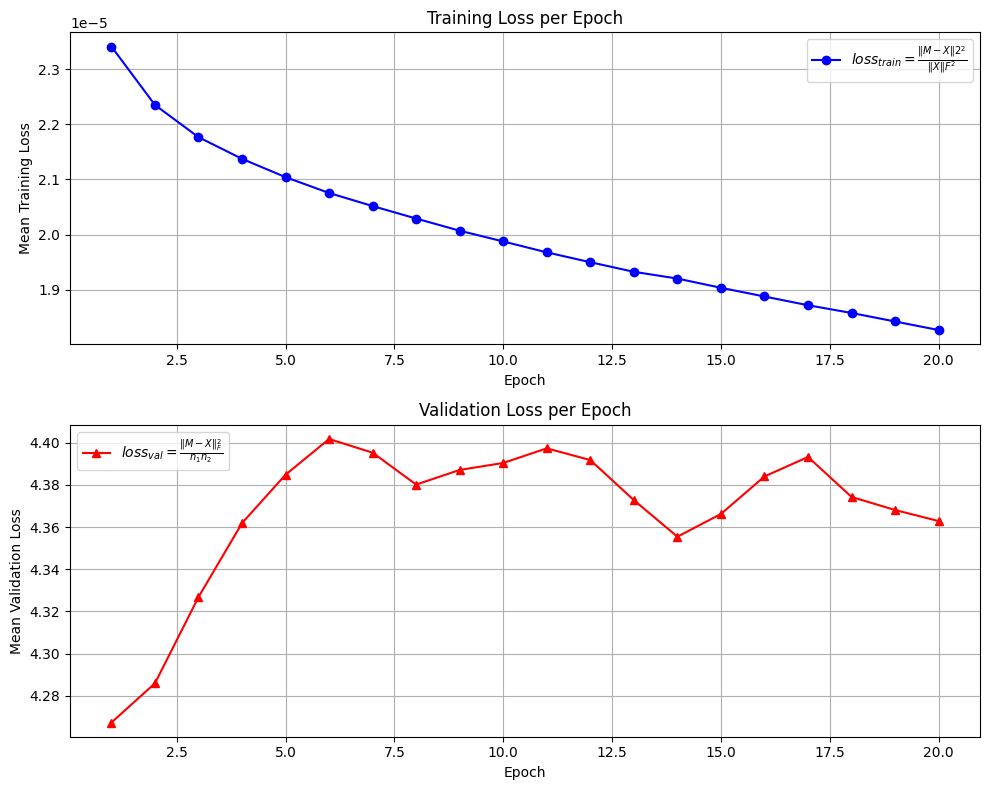
\includegraphics[width=\textwidth]{output_30_06}
    \caption{Training and validation loss for 30\% sampling rate and 6 SNR}
    \label{fig:output_30_06}
\end{figure}

\begin{figure}[htbp]
    \centering
    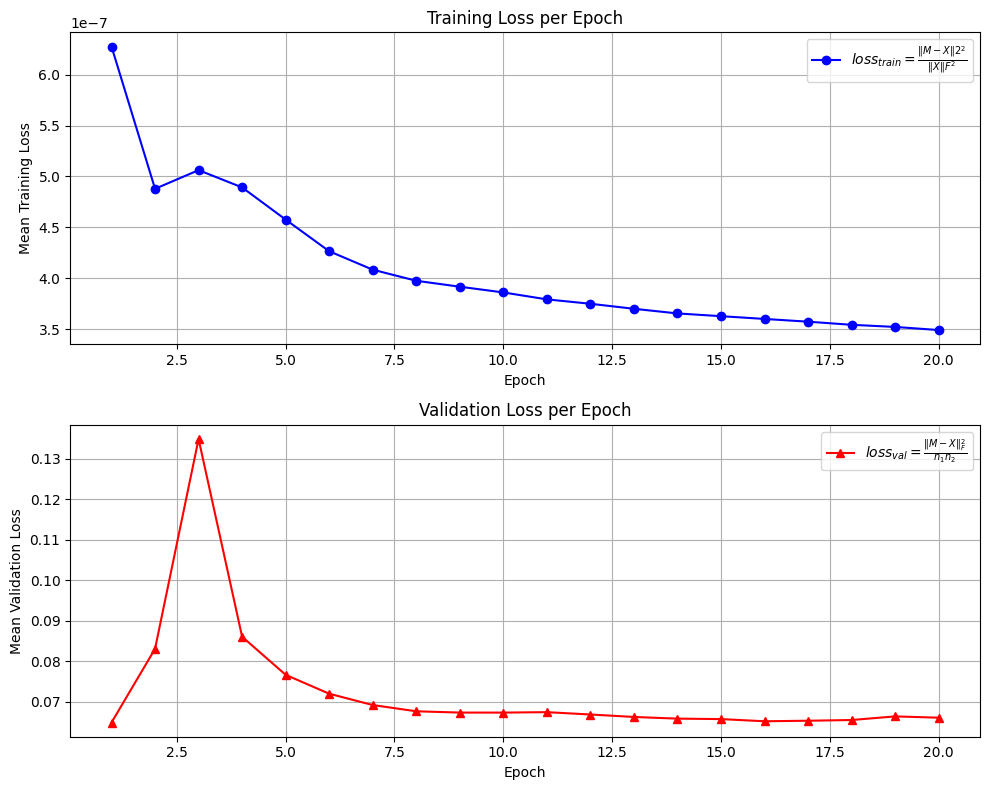
\includegraphics[width=\textwidth]{output_80_05}
    \caption{Training and validation loss for 80\% sampling rate and 5 SNR}
    \label{fig:output_80_05}
\end{figure}

\begin{figure}[htbp]
    \centering
    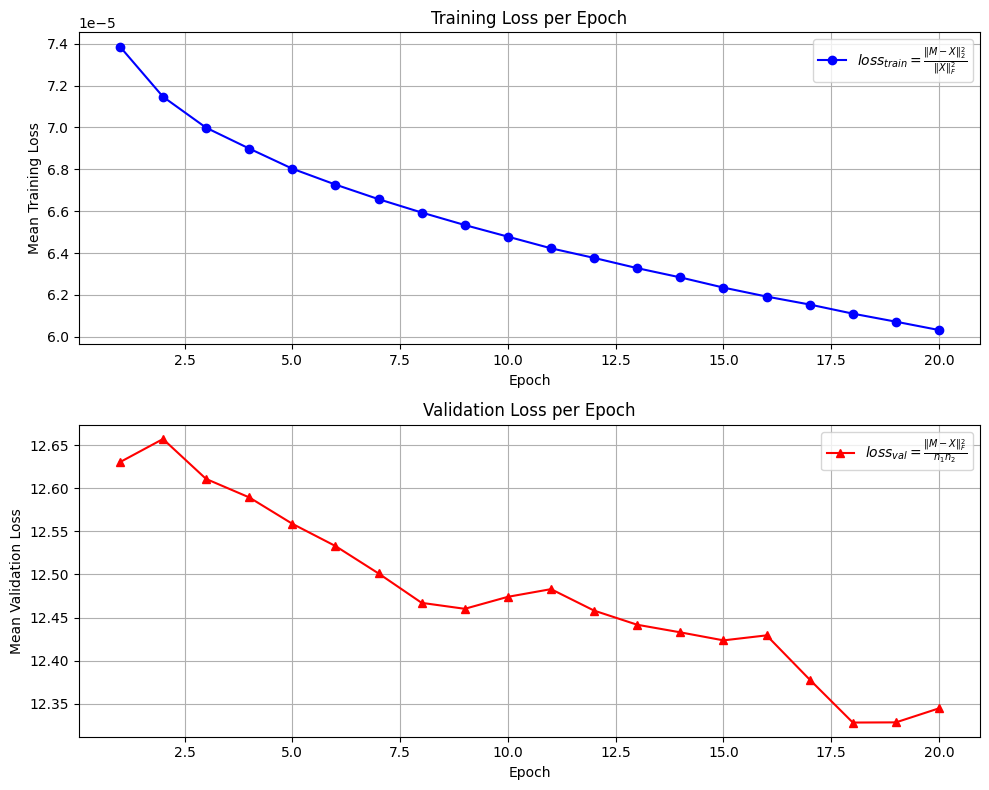
\includegraphics[width=\textwidth]{output_20_03}
    \caption{Training and validation loss for 20\% sampling rate and 3 SNR}
    \label{fig:output_20_03}
\end{figure}

\begin{figure}[htbp]
    \centering
    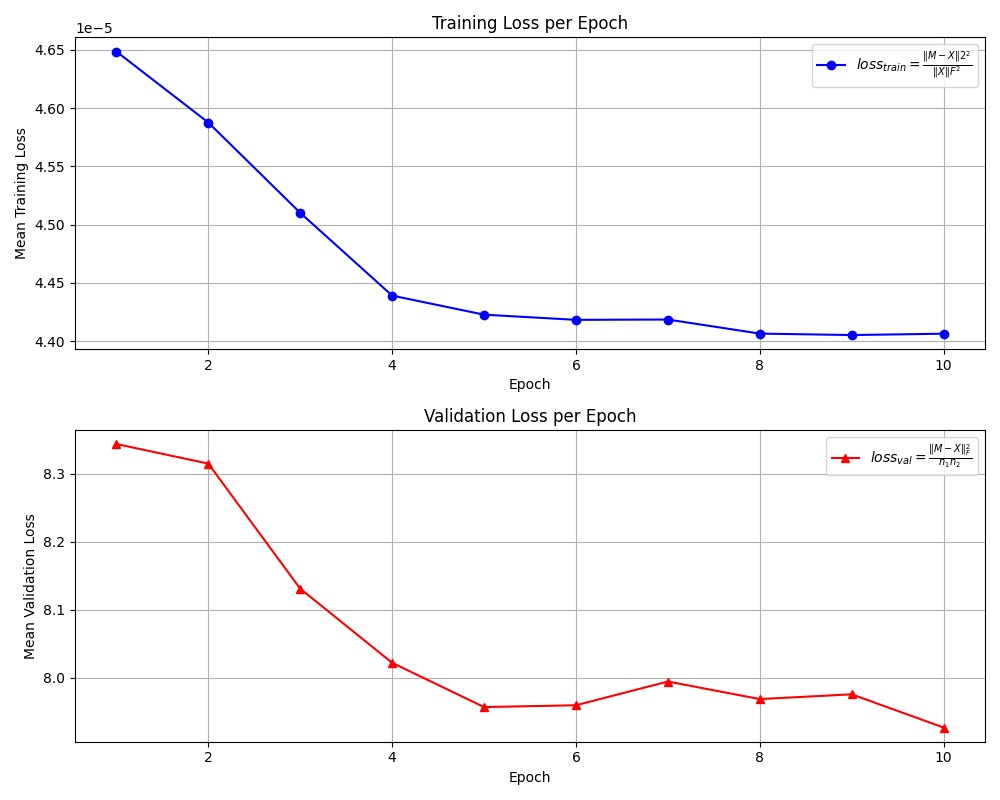
\includegraphics[width=\textwidth]{output_80_09}
    \caption{Training and validation loss for 80\% sampling rate and 9 SNR}
    \label{fig:output_80_09}
\end{figure}

Given this inherent unpredictability of ConvHuberMC-Net, we decided to exclude it from further analyses (on image inpainting and on matrices of shape (400 \(\times\) 500)) until we can pin the issue down. Our hypothesis is that the issue is related to the smooth and convex nature of matrix factorization algorithms and their operations and how they might not, therefore, be the optimal kind of algorithms for deep unfolding, unlike algorithms involving non-smooth operations, e.g., ALM. This also explains the fact that rarely anyone has unfolded algorithms involving matrix factorization so far. Before shelving the model, we did attempt to address the uncertainty in performance by learning the pseudoinverse that appears in Huber regression. However, this led to even more problematic performance, as now the model became completely insensitive to changes in sampling rate and SNR. For example, the two extreme combinations of 20\% sampling rate and 3 SNR and 80\% sampling rate with 9 SNR have nearly identical ranges for the training and validation losses, as shown in Figure \ref{fig:output_20_03} and Figure \ref{fig:output_80_09}. We ultimately dismissed this idea and, though we have shared a case of ConvHuberMC-Net outperforming the rest of the algorithms, it should be noted that this is not the case for all cases.

% When you are done with these 4 graphs, come to the fact that although our model especially HuberMC is sus at some times (for e.g share its loss patterns for 30% (DB 6 - ve light) sampling rate - up and down val loss), but at other times it has also performed normally. Here you can share its performance at (80% with 5 DB +ve light) sampling where the loss is decreasing with increase in DB generally speaking. Intepret both cases. Conclude this section by saying that due to the unpredictability and unsatisfactory performance of hubermc we choose not to go ahead with it while doing experimentation on image inpainting. Maybe link the reason of its sus performance to the nature of matrix factorization algorithms which are smooth and convex most of the time and hence the DNN might have some troubles in terms in learning when it comes to smooth operations such as found in matrix factorization as compared to non-smooth operations found in ALM type approaches.
% Considering these sus cases, we also considered learning the psuedoinverse as well however for some reason (if you can come up with some to likh dena) the loss trajectories became indifferent to the sampling and db combination and for each combo the val loss was in between 7 and 8. Here show the pic/graphs at 80% 9DB vs 20% 3DB and show both are in similar ranges in terms of val loss. Hence we dismissed this idea. Hence although at first it seems like it has performed way better for the 20% case, its not following the expected pattern for other combos. We finish HuberMC here. 
% ConvMC on the other hand has shown tremendous results beating many of the algorithms in synthetic 150 x 300, hence we go ahead and test it with all other algorithms in image inpainting. Suprisingly, we observed that although we did not take into account sort of noise in the $L$ update or neither the lagrange multiplier update, it still was able to after training on white-noise and GMM noise perform exceedingly well. This may prove our previous hypothesis where we claimed that the 'learning' feature of DNN might still be able to handle 'seeimgly' out - of - distribution tasks.
% Before ending the discussion on the first graph comment how the seemingly state of the art method L0-BCD has not performed to its expectations and other algorithms such as M-est are beating it. This suggests that these methods are signficantly related with the matrix dimension size with no general trend. This will be proven later in the next graph when we show the results for 400 x 500 synthetic. 
% For 400 x 500 synthetic just go ahead and intepret the results as they are but dont forget to mention how the above results where L0-BCD was not performing relatively better than M-est now its 10x better. Breifly mention again how we skipped hubermc in this graph due to its unpredictable and unsatisfactory performance. Share only one case of 20% and 3DB where the val loss is increasing but train loss is decreasing. 
The case for matrices of shape (400 \(\times\) 500) is shown in Figure \ref{fig:mse_snr_400_500}. It is obvious that merely changing the shape of matrices involved in the optimization process resulted in noticeable changes. \(\ell_0\)-BCD, which was far from the top, now outperforms every other algorithm by a big margin. It is uniformly followed by M-estimation, \(\ell_p\)-reg, \(\ell_p\)-ADMM, ORMC, and ConvMC-Net. This small yet important finding regarding the significance of matrix shape in matrix completion problems also requires further investigation.

After the detailed experimentation on synthetic dataset, we transitioned to image inpainting. The results for both $150 \times 300$ and $400 \times 500$ are summarized in Table \ref{tab:psnr_ssim_150_300} and \ref{tab:psnr_ssim_400_500}. From Table \ref{tab:psnr_ssim_150_300} we observe that surprisingly $\ell_{p}$-reg takes the lead in almost all of the combinations with second place going to either $\ell_{0}$-BCD or M-Estimation. This might suggest that the parameters such as $\sigma$ required for $\ell_{0}$-BCD algorithm i.e. which controls the outlier presence in the matrix needs to be fine-tuned because its very unlikely it performs not the best among all others considering its complete dominance in for the matrix size $400 \times 500$ as shown in \ref{tab:psnr_ssim_400_500}. Furthermore, if we start to take into account the inference times of each of these methods, $\ell_{0}$-BCD and M-estimation are at the top with $\ell_{p}$-reg or $\ell_{p}$-ADMM taking nearly $100\times$ of the time to achieve similar performance for or lower performance in the case of $\ell_{p}$-ADMM. 

We also observe regarding our proposed model, ConvMC-Net a poor performance in all combinations despite its seemingly overwhelming inference time. This can be attributed to the fact that we discussed in detail in Section 2 and 3 that such PCP methods aren not flexible to deal with impulsive noises, even more so if the objective function does not incorporate even white noise. However, we do observe of what one can deem to be anomaly at Image 8 of $150 \times 300$ dimensions. The PSNR is almost in the range of $40$'s and SSIM is nearly $0.9$ something which is way greater than the rest of the values. 

However, to test whether this was indeed an anomaly, we look at the below Table \ref{tab:psnr-ssim} which shows only ConvMC-Net's result for sampling rate $20\%$ and DB as %5.0%
\begin{table}[h]
\centering
\begin{tabular}{|c|c|c|}
\hline
\text{Image} & \text{PSNR} & \text{SSIM} \\
\hline
1 & 32.98 & 0.57 \\
2 & 33.41 & 0.61 \\
3 & 32.83 & 0.52 \\
4 & 33.40 & 0.58 \\
5 & 33.50 & 0.60 \\
6 & 33.96 & 0.63 \\
7 & 33.53 & 0.59 \\
8 & 34.75 & 0.63 \\
\hline
\end{tabular}
\caption{PSNR and SSIM values for ConvMC-Net with 20\% sampling rate and DB 5.0}
\label{tab:psnr-ssim}
\end{table}
As if this is not surprising enough, we observe similar results in most of the combinations even for the case of $400 \times 500$. This result, we believe is still not to be taken as completely trustworthy and requires further investigation. This is because, if the same model does not perform even close to other algorithms in the synthetic dataset, it should be very unlikely it overwhelms for the case of image inpainting experimentation.
% Note: For the image inpainting intepretation, use the current combo in the table i.e. 5DB and 50% sampling rate and attach convmc  results to the table for both 150 x 300 and 400 x 500. Here comment how seemingly convmc is performing way worse than other algorithms but somehow (if you can come up with any scientific reason then use it) for other combos its is dominating all other algorithms with PSNR in ranges of 35 - 45 and ssim in ranges of 0.8-0.95 etc. (You can even show a small table for it as well.) And comment on the L-BCD performance difference between 150 x 300 and 400 x 500 similar to the synthetic one. But an additonal suprise here is that lp-reg is dominating the 150 x 300 section and its in close second for 400 x 500 even beating M-estimation is some combos which was not the case for synthetic.